\section{公司管理概况}
\subsection{高层简介}

\begin{table}[H]
  \centering
  \caption{高层简介}
    \begin{tabular}{|c|c|c|}
    \hline
    \textcolor[rgb]{ .298,  .282,  .239}{姓名} & \textcolor[rgb]{ .298,  .282,  .239}{学历} & \textcolor[rgb]{ .298,  .282,  .239}{专业} \\
    \hline
    \textcolor[rgb]{ .298,  .282,  .239}{陈洪璞} & \textcolor[rgb]{ .298,  .282,  .239}{中国人民大学本科在读} & \textcolor[rgb]{ .298,  .282,  .239}{信息管理与信息系统} \\
    \hline
    \textcolor[rgb]{ .298,  .282,  .239}{汪圣灵} & \textcolor[rgb]{ .298,  .282,  .239}{北京航空航天大学本科在读} & \textcolor[rgb]{ .298,  .282,  .239}{计算机科学与技术} \\
    \hline
    \textcolor[rgb]{ .298,  .282,  .239}{汪军水} & \textcolor[rgb]{ .298,  .282,  .239}{清华大学本科在读} & \textcolor[rgb]{ .298,  .282,  .239}{工程物理} \\
    \hline
    \end{tabular}%
  \label{tab:gaocengjeshao}%
\end{table}%

\subsection{高层分工}
高层分工如下:
\begin{figure}[H]
	\centering
	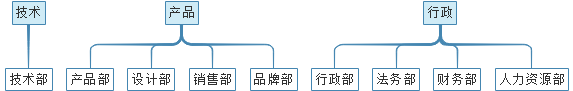
\includegraphics[width=0.9\columnwidth]{figures/high_level_division}
	%  \setlength{\abovecaptionskip}{0pt}
	%  \setlength{\belowcaptionskip}{-20pt}
	\caption{高层分工}
	\label{fg:high_level_division}
\end{figure}

\subsection{管理体系}
\subsubsection{课程管理体系}\

\paragraph{兼职课程运营管理}\

为开拓广阔的课程教师来源,我们公司会在必要的时期大量招收实习生,对兼职找老师的同学,我们的要求是要有一定的学生工作经验,若表现出色,则考虑吸收到创业团队。

\paragraph{课程教师管理}\

对课程教师,我们计划的筛选比例是20:1,同时为防止教师与其他在线教育平台合作,我们考虑两种方式,一种找专业非常好的大学在读生,未来就业方向不在教育领域,避免了冲突与竞争,第二种,课程收益与老师分成的形式,长期留住优秀的老师。若出现人气高的老师与其他在线教育平台合作,要第一时间找到可替代的老师。

\paragraph{课程制作时间控制}\

在课程市场调查结束之后,前期要预留一个月筛选老师,两个月进行宣传,保证有足够的时间应对突发情况。

\subsubsection{部门合作管理}\

各部门之间需要紧密合作,首先,以产品部为核心,产品部三大组成相互协调合作,共同规划产品方向与形式;以用户友好为目标,不断从课程品质和用户友好度方面完善平台产品。充分发挥高校兼职同学的创造力和想象力,同时,在法务和财务方面细化分工,防止出现意外情况。需要专人专职负责。

每周进行各部门理事会,每月部门负责人给全员汇报工作,统一思想。

\subsection{人事管理}
\subsubsection{管理思想}\

优良科学管理的前提是确定和贯彻正确先进的管理思想。我们将采取张瑞敏先生 “众谋独断、详虑力行”的管理思想。重视个人的发展,尊重个人价值, 但也同时强调各职能部门相互协调合作,求得公司的整体发展,实现最优效果。

\subsubsection{管理决策}\

公司初期的管理团队主要由创业团队人员组成。团队成员都是具本科在读的大学生,具有相关的专业知识和高效的执行力,将为公司制定切实可行的决策,执行最有效率的任务。在获得风险投资后,投资家自然也成为我们的公司管理顾问,我们还将邀请具有各专业技术及管理经验的人员加入,并担任重要职务。

\subsubsection{管理理念}\

关心员工成长、强化执行能力、追求高效和谐、平衡激励约束。

\paragraph{关心员工成长}\

重视员工的兴趣和专长,以良好的工作条件、完善的员工培训计划、职业生涯通道设计促进员工个人职业发展;重视企业文化管理,以健康简单的人际关系、严肃活泼的工作气氛、畅快透明的沟通方式,促进员工满意度的不断提高,使员工保持与企业同步成长的快乐;激发员工潜能,追求个人与公司共同成长。作为个人要有先付出的意识,甘于为团队奉献智慧和勤奋,以优秀的团队成就个人的优秀。
\paragraph{强化执行能力}\

再好的研究策划,没有好的执行就会成为空谈。强力执行是创业在管理上的核心原则之一;良好的执行力,要依靠优秀的机制、规范的制度、精诚的合作、有效的激励、感人的榜样,但最重要的,要依靠每位创业人对公司的热爱和对工作的负责精神;
\paragraph{追求高效和谐}\

根据公司发展阶段和业务变化,动态优化企业的管理,形成和谐有序的内部环境;在高效与和谐的环境下,坚持结果导向的管理原则,有效支持公司经营目标的实现。
\paragraph{平衡激励约束}\

根据工作贡献和成果价值, 形成差异化的激励机制,有效激发员工的主观能动性和创造性; 强调激励与约束相结合、保持平衡有度,为实现内部管理提供有力保障。

\paragraph{充分价值体现}\

充分发挥每一名员工的人脉资源与隐性知识,在人脉资源方面,配合课程部教师的合格找寻,成功介绍老师者将会有专门的奖励机制进行奖励;在个人隐性知识方面,充分体现员工优势,鼓励对显性知识的转化,同样有奖励机制。





